\documentclass{standalone}
\usepackage{tikz}
\usetikzlibrary{patterns, positioning}


\begin{document}
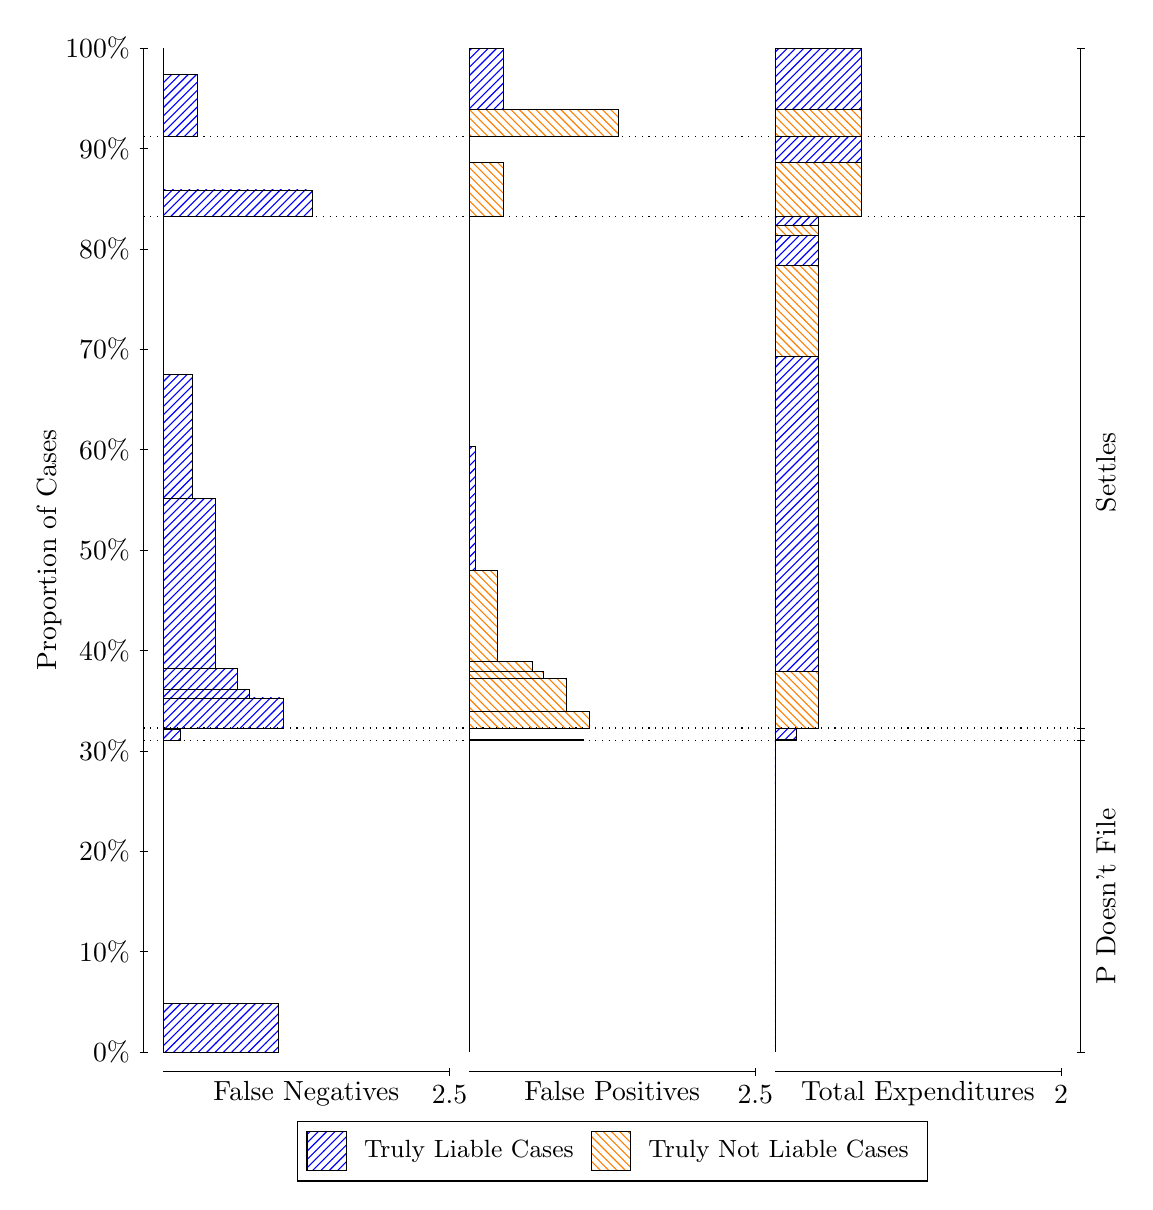
\begin{tikzpicture}
\draw[black, very thin] (1.5,1.75) -- (1.5,14.5);
\node[rotate=90, text=black, anchor=center] at (0.3, 8.125) {Proportion of Cases};
\draw[black, very thin] (1.45,1.75) -- (1.55,1.75);
\node[text=black, anchor=east] at (1.45, 1.75) {0\%};
\draw[black, very thin] (1.45,3.025) -- (1.55,3.025);
\node[text=black, anchor=east] at (1.45, 3.025) {10\%};
\draw[black, very thin] (1.45,4.3) -- (1.55,4.3);
\node[text=black, anchor=east] at (1.45, 4.3) {20\%};
\draw[black, very thin] (1.45,5.575) -- (1.55,5.575);
\node[text=black, anchor=east] at (1.45, 5.575) {30\%};
\draw[black, very thin] (1.45,6.85) -- (1.55,6.85);
\node[text=black, anchor=east] at (1.45, 6.85) {40\%};
\draw[black, very thin] (1.45,8.125) -- (1.55,8.125);
\node[text=black, anchor=east] at (1.45, 8.125) {50\%};
\draw[black, very thin] (1.45,9.4) -- (1.55,9.4);
\node[text=black, anchor=east] at (1.45, 9.4) {60\%};
\draw[black, very thin] (1.45,10.675) -- (1.55,10.675);
\node[text=black, anchor=east] at (1.45, 10.675) {70\%};
\draw[black, very thin] (1.45,11.95) -- (1.55,11.95);
\node[text=black, anchor=east] at (1.45, 11.95) {80\%};
\draw[black, very thin] (1.45,13.225) -- (1.55,13.225);
\node[text=black, anchor=east] at (1.45, 13.225) {90\%};
\draw[black, very thin] (1.45,14.5) -- (1.55,14.5);
\node[text=black, anchor=east] at (1.45, 14.5) {100\%};

\draw[black, very thin] (13.4,1.75) -- (13.4,14.5);
\draw[black, very thin] (13.35,1.75) -- (13.45,1.75);
\node[anchor=west] at (13.35, 1.75) {};
\draw[black, very thin] (13.35,5.7041) -- (13.45,5.7041);
\node[anchor=west] at (13.35, 5.7041) {};
\draw[black, very thin] (13.35,5.8643) -- (13.45,5.8643);
\node[anchor=west] at (13.35, 5.8643) {};
\draw[black, very thin] (13.35,12.362) -- (13.45,12.362);
\node[anchor=west] at (13.35, 12.362) {};
\draw[black, very thin] (13.35,13.38) -- (13.45,13.38);
\node[anchor=west] at (13.35, 13.38) {};
\draw[black, very thin] (13.35,14.5) -- (13.45,14.5);
\node[anchor=west] at (13.35, 14.5) {};

\draw[black, very thin, pattern color=blue, pattern=north east lines] (1.75,1.75) rectangle (3.2033,2.3646);
\draw[black, very thin, pattern color=orange, pattern=north west lines] (1.75,2.3646) rectangle (1.75,5.7041);
\draw[black, very thin, pattern color=blue, pattern=north east lines] (1.75,5.7041) rectangle (1.968,5.8493);
\draw[black, very thin, pattern color=orange, pattern=north west lines] (1.75,5.8493) rectangle (1.75,5.8643);
\draw[black, very thin, pattern color=blue, pattern=north east lines] (1.75,5.8643) rectangle (3.276,6.248);
\draw[black, very thin, pattern color=blue, pattern=north east lines] (1.75,6.248) rectangle (2.84,6.3582);
\draw[black, very thin, pattern color=blue, pattern=north east lines] (1.75,6.3582) rectangle (2.6947,6.6195);
\draw[black, very thin, pattern color=blue, pattern=north east lines] (1.75,6.6195) rectangle (2.404,8.7828);
\draw[black, very thin, pattern color=blue, pattern=north east lines] (1.75,8.7828) rectangle (2.1133,10.36);
\draw[black, very thin, pattern color=orange, pattern=north west lines] (1.75,10.36) rectangle (1.75,12.362);
\draw[black, very thin, pattern color=blue, pattern=north east lines] (1.75,12.362) rectangle (3.6393,12.698);
\draw[black, very thin, pattern color=orange, pattern=north west lines] (1.75,12.698) rectangle (1.75,13.38);
\draw[black, very thin, pattern color=blue, pattern=north east lines] (1.75,13.38) rectangle (2.186,14.164);
\draw[black, very thin, pattern color=orange, pattern=north west lines] (1.75,14.164) rectangle (1.75,14.5);
\draw[black, very thin, pattern color=orange, pattern=north west lines] (5.6333,1.75) rectangle (5.6333,5.0895);
\draw[black, very thin, pattern color=blue, pattern=north east lines] (5.6333,5.0895) rectangle (5.6333,5.7041);
\draw[black, very thin, pattern color=orange, pattern=north west lines] (5.6333,5.7041) rectangle (7.0867,5.7191);
\draw[black, very thin, pattern color=blue, pattern=north east lines] (5.6333,5.7191) rectangle (5.6333,5.8643);
\draw[black, very thin, pattern color=orange, pattern=north west lines] (5.6333,5.8643) rectangle (7.1593,6.073);
\draw[black, very thin, pattern color=orange, pattern=north west lines] (5.6333,6.073) rectangle (6.8687,6.4922);
\draw[black, very thin, pattern color=orange, pattern=north west lines] (5.6333,6.4922) rectangle (6.578,6.5862);
\draw[black, very thin, pattern color=orange, pattern=north west lines] (5.6333,6.5862) rectangle (6.4327,6.7135);
\draw[black, very thin, pattern color=orange, pattern=north west lines] (5.6333,6.7135) rectangle (5.9967,7.8669);
\draw[black, very thin, pattern color=blue, pattern=north east lines] (5.6333,7.8669) rectangle (5.706,9.4437);
\draw[black, very thin, pattern color=blue, pattern=north east lines] (5.6333,9.4437) rectangle (5.6333,12.362);
\draw[black, very thin, pattern color=orange, pattern=north west lines] (5.6333,12.362) rectangle (6.0693,13.044);
\draw[black, very thin, pattern color=blue, pattern=north east lines] (5.6333,13.044) rectangle (5.6333,13.38);
\draw[black, very thin, pattern color=orange, pattern=north west lines] (5.6333,13.38) rectangle (7.5227,13.716);
\draw[black, very thin, pattern color=blue, pattern=north east lines] (5.6333,13.716) rectangle (6.0693,14.5);
\draw[black, very thin, pattern color=orange, pattern=north west lines] (9.5167,1.75) rectangle (9.5167,5.0895);
\draw[black, very thin, pattern color=blue, pattern=north east lines] (9.5167,5.0895) rectangle (9.5167,5.7041);
\draw[black, very thin, pattern color=orange, pattern=north west lines] (9.5167,5.7041) rectangle (9.7892,5.7191);
\draw[black, very thin, pattern color=blue, pattern=north east lines] (9.5167,5.7191) rectangle (9.7892,5.8643);
\draw[black, very thin, pattern color=orange, pattern=north west lines] (9.5167,5.8643) rectangle (10.062,6.5862);
\draw[black, very thin, pattern color=blue, pattern=north east lines] (9.5167,6.5862) rectangle (10.062,10.587);
\draw[black, very thin, pattern color=orange, pattern=north west lines] (9.5167,10.587) rectangle (10.062,11.741);
\draw[black, very thin, pattern color=blue, pattern=north east lines] (9.5167,11.741) rectangle (10.062,12.125);
\draw[black, very thin, pattern color=orange, pattern=north west lines] (9.5167,12.125) rectangle (10.062,12.252);
\draw[black, very thin, pattern color=blue, pattern=north east lines] (9.5167,12.252) rectangle (10.062,12.362);
\draw[black, very thin, pattern color=orange, pattern=north west lines] (9.5167,12.362) rectangle (10.607,13.044);
\draw[black, very thin, pattern color=blue, pattern=north east lines] (9.5167,13.044) rectangle (10.607,13.38);
\draw[black, very thin, pattern color=orange, pattern=north west lines] (9.5167,13.38) rectangle (10.607,13.716);
\draw[black, very thin, pattern color=blue, pattern=north east lines] (9.5167,13.716) rectangle (10.607,14.5);
\draw[black, dotted] (1.5,5.7041) -- (13.4,5.7041);
\draw[black, dotted] (1.5,5.8643) -- (13.4,5.8643);
\draw[black, dotted] (1.5,12.362) -- (13.4,12.362);
\draw[black, dotted] (1.5,13.38) -- (13.4,13.38);
\draw[black, very thin] (1.75,1.5) -- (5.3833,1.5);
\node[text=black, anchor=north] at (3.5667, 1.5) {False Negatives};
\draw[black, very thin] (5.3833,1.45) -- (5.3833,1.55);
\node[text=black, anchor=north] at (5.3833, 1.45) {2.5};

\draw[black, very thin] (5.6333,1.5) -- (9.2667,1.5);
\node[text=black, anchor=north] at (7.45, 1.5) {False Positives};
\draw[black, very thin] (9.2667,1.45) -- (9.2667,1.55);
\node[text=black, anchor=north] at (9.2667, 1.45) {2.5};

\draw[black, very thin] (9.5167,1.5) -- (13.15,1.5);
\node[text=black, anchor=north] at (11.333, 1.5) {Total Expenditures};
\draw[black, very thin] (13.15,1.45) -- (13.15,1.55);
\node[text=black, anchor=north] at (13.15, 1.45) {2};

\node[text=black, centered, rotate=90] at (13.72, 3.7271) {P Doesn't File};

\node[text=black, centered, rotate=90] at (13.72, 9.1132) {Settles};



\draw (7.449999999999999,1.5) node[draw=none] (baseCoordinate) {};
\begin{scope}[align=center]
        \matrix[scale=0.5, draw=black, below=0.5cm of baseCoordinate, nodes={draw}, column sep=0.1cm]{
            \node[rectangle, draw, minimum width=0.5cm, minimum height=0.5cm, pattern color=blue, pattern=north east lines] {}; &
            \node[draw=none, font=\small, text=black] (B) {Truly Liable Cases}; &
            \node[rectangle, draw, minimum width=0.5cm, minimum height=0.5cm, pattern color=orange, pattern=north west lines] {}; &
            \node[draw=none, font=\small, text=black] (B) {Truly Not Liable Cases}; \\
            };
\end{scope}

\end{tikzpicture}
\end{document}